%
% Template for RBIE papers in LaTeX
%

% The above language combination is for this template document only.
% You should use one of the following:
\documentclass[english, spanish, brazilian]{RBIEarticle} % for papers in portuguese
%\documentclass[brazilian, spanish, english]{RBIEarticle} % for papers in english
%\documentclass[brazilian, english, spanish]{RBIEarticle} % for papers in spanish

% Papers in Portuguese or Spanish may require the following lines:
\usepackage[utf8]{inputenc} % chooses UTF-8 as the main character set
\usepackage[T1]{fontenc} % for correct syllable separation in accented words

% The next two statements are needed for the example table in this document
% (i.e. you don't necessarily need them in your own paper)
\usepackage{colortbl}
\definecolor{gray}{gray}{.8}

% Citations and references (Biblatex)
\usepackage[style=apa]{biblatex}
\usepackage{csquotes}

\usepackage{longtable}
\usepackage{booktabs}
\usepackage{tabularx}
\usepackage{float}

\addbibresource{references.bib}

% Here goes the paper main title
\title{Previsão da evasão de alunos de cursos de computação nas instituições federais do Brasil usando Aprendizado de Máquina}

% If the manuscript is written in English, then this element must be removed.
\titleinenglish{Predicting student dropout rates in computing courses in Brazil's federal institutions using Machine Learning}

% If the manuscript is written in English, then this element must be removed.
\titleinspanish{Predicción de las tasas de abandono estudiantil en los cursos de informática de las instituciones federales de Brasil mediante el aprendizaje automático}

% Here goes the paper author information (repeat for two or more authors)
\author{%
	\parbox{8cm}{%
		Gustavo Ferreira Botelho de Sena\\
		Graduando em Sistemas de Informação na Escola de Artes, Ciências e Humanidades da Universidade de São Paulo (EACH-USP) \\
		gustavoferreirasena@usp.br
	}
    \vspace{1cm}
    \quad
	\parbox{8cm}{%
		Renan Moura Nascimento\\
		Graduando em Sistemas de Informação na Escola de Artes, Ciências e Humanidades da Universidade de São Paulo (EACH-USP) \\
		renan.moura@usp.br
	}
        \newline
        \parbox{8cm}{%
		Rony dos Santos Teles\\
		Graduando em Sistemas de Informação na Escola de Artes, Ciências e Humanidades da Universidade de São Paulo (EACH-USP) \\
		rony.teles@usp.br
	}
        \quad
        \vspace{1cm}
        \parbox{8cm}{%
		Silvio Marcelo F. Bertoldo\\
		Graduando em Sistemas de Informação na Escola de Artes, Ciências e Humanidades da Universidade de São Paulo (EACH-USP) \\
		silvio.bertoldo@usp.br
	}
}

\Submission{20/10/2025}
% >>> A ser feito depois <<<
%\First_round_notif{dd/Mmm/yyyy}
%\New_version{dd/Mmm/yyyy}
%\Second_round_notif{dd/Mmm/yyyy}
%\Camera_ready{dd/Mmm/yyyy}
%\Edition_review{dd/Mmm/yyyy}
%\Available_online{dd/Mmm/yyyy}
%\Published{dd/Mmm/yyyy}

% Here goes the page heading information
\heading{Sena, G. F. B., Nascimento, R. M., Teles, R. S., Bertoldo, S. M. F.	\\
Bertoldo et al.
}{RBIE v.VV – 2025}

% And finally here goes the citation information
% >>> A ser feito depois <<<
\citeas{Sena, G. F. B., Nascimento, R. M., Teles, R. S., Bertoldo, S. M. F. (2025). Previsão da evasão de alunos de cursos de computação nas instituições federais do Brasil usando Aprendizado de Máquina. Revista Brasileira de Informática na Educação, vol, pp-pp. https://doi.org/10.5753/rbie.yyyy.id}

%====================================================================
%\hyphenpenalty=10000
%\setcounter{page}{01}

\begin{document}
\maketitle

% If the manuscript is written in English, then this element must be removed.
\begin{otherlanguage}{brazilian}
\begin{abstract}
A evasão de alunos no ensino superior é um desafio que traz impactos às políticas governamentais, às instituições de ensino, aos estudantes evadidos e à sociedade. Este estudo tem como objetivo aplicar e comparar diferentes técnicas de aprendizado de máquina na predição da evasão em cursos de computação no Brasil, utilizando os microdados da Plataforma Nilo Peçanha das instituições federais brasileiras. O processo metodológico compreende as etapas de coleta, pré-processamento, modelagem e avaliação, considerando variáveis demográficas, socioeconômicas e acadêmicas. Para o problema, serão empregados algoritmos supervisionados como Regressão Logística, Árvores de Decisão, Random Forest, K-Nearest Neighbors, Naïve Bayes, Support Vector Machine e Redes Neurais. A performance dos modelos será analisada a partir de métricas padrão, incluindo acurácia, precisão, recall, F1-Score e área sob a curva (AUC). Espera-se identificar o algoritmo com melhor desempenho, contribuindo para um melhor entendimento deste fenômeno complexo visando apoiar o desenvolvimento de estratégias de retenção estudantil mais eficazes.
\keywords EEvasão estudantil, Ensino superior, Universidades federais, Brasil, Aprendizado de máquina, Mineração de dados, Classificação binária, Algoritmos supervisionados, Regressão Logística, Random Forest, Redes Neurais.
\end{abstract}
\end{otherlanguage}

\newpage
\begin{otherlanguage}{english}
\begin{abstract}
Student dropout in higher education is a challenge that impacts government policies, educational institutions, students, and society as a whole. This study aims to apply and compare different machine learning techniques to predict dropout rates in computing programs in Brazil, using microdata from the Nilo Peçanha Platform of Brazilian federal institutions. The methodological process comprises the stages of data collection, pre-processing, modeling, and evaluation, considering demographic, socioeconomic, and academic variables. Supervised algorithms such as Logistic Regression, Decision Trees, Random Forest, K-Nearest Neighbors, Naive Bayes, Support Vector Machines, and Neural Networks will be employed to solve this problem. The models' performance will be analyzed using standard metrics, including accuracy, precision, recall, F1-score, and area under the curve (AUC). The aim is to identify the best-performing algorithm, contributing to a better understanding of this complex phenomenon and supporting the development of more effective student retention strategies.
\keywords SStudent Dropout, Higher Education, Federal Universities, Brazil, Machine Learning, Data Mining, Binary Classification, Supervised Algorithms, Logistic Regression, Random Forest, Neural Networks.
\end{abstract}
\end{otherlanguage}

% If the manuscript is written in English, then this element must be removed.
\begin{otherlanguage}{spanish}
\begin{abstract}
La deserción estudiantil en la educación superior es un desafío que impacta las políticas gubernamentales, las instituciones educativas, los estudiantes y la sociedad en su conjunto. Este estudio tiene como objetivo aplicar y comparar diferentes técnicas de aprendizaje automático para predecir las tasas de deserción en programas de informática en Brasil, utilizando microdatos de la Plataforma Nilo Peçanha de instituciones federales brasileñas. El proceso metodológico comprende las etapas de recolección de datos, preprocesamiento, modelado y evaluación, considerando variables demográficas, socioeconómicas y académicas. Se emplearán algoritmos supervisados como Regresión Logística, Árboles de Decisión, Bosque Aleatorio, K-Vecinos Más Cercanos, Bayes Ingenuo, Máquinas de Vectores de Soporte y Redes Neuronales para resolver este problema. El desempeño de los modelos se analizará utilizando métricas estándar, incluyendo exactitud, precisión, recuperación, puntuación F1 y área bajo la curva (AUC). El objetivo es identificar el algoritmo con mejor desempeño, contribuyendo a una mejor comprensión de este complejo fenómeno y apoyando el desarrollo de estrategias de retención estudiantil más efectivas.
\keywords AAbandono estudiantil, Educación superior, Universidades federales, Brasil, Aprendizaje automático, Minería de datos, Clasificación binaria, Algoritmos supervisados, Regresión logística, Bosque aleatorio, Redes neuronales.
\end{abstract}
\end{otherlanguage}

\pagebreak

%===================================================================

\section{Introdução}
A evasão de alunos é um problema persistente e multifacetado que impacta instituições de ensino superior em todo o mundo, com impactos sociais e econômicos. No Brasil, a situação é particularmente preocupante: uma parcela significativa dos estudantes não conclui os cursos em que ingressam, resultando em prejuízos financeiros para as instituições, perda de recursos públicos investidos em políticas educacionais e diminuição da oferta de profissionais qualificados para o mercado de trabalho.  Conseguir identificar os fatores que levam à evasão estudantil é um desafio estratégico para o planejamento institucional e para a formulação de políticas públicas voltadas à permanência dos alunos.

As abordagens tradicionais de análise estatística, embora de grande relevância, apresentam limitações diante da crescente complexidade e volume de dados disponíveis. Nesse cenário, a mineração de dados e o aprendizado de máquina destacam-se, capazes de explorar grandes bases de informação e ajudar a detectar padrões que possam indicar possível evasão. Tais técnicas entregariam, então, um grande poder às instituições, permitindo a elas conhecer de antemão quais estudantes estariam em risco de evasão, permitindo desenhar políticas e estratégias que fomentassem a permanência estudantil.

Diversos estudos nacionais e internacionais têm explorado o uso de modelos preditivos aplicados à evasão, empregando algoritmos de classificação como Regressão Logística, Árvores de Decisão e Random Forest. Grande parte dessas pesquisas utiliza dados do Censo da Educação Superior do Inep, que, embora abrangentes, não contemplam especificidades dos contextos institucionais e cursos. O presente trabalho diferencia-se ao fazer uso dos microdados da Plataforma Nilo Peçanha (PNP), considerada a principal base sobre a Rede Federal de Educação Profissional, Científica e Tecnológica (RFEPCT) brasileira, permitindo um bom enfoque ao problema da evasão em cursos de computação brasileiros de nível superior.

Desta forma, este estudo busca aplicar e avaliar comparativamente diferentes algoritmos de aprendizado supervisionado (Regressão Logística, Árvores de Decisão, Random Forest, K-Nearest Neighbors, Naïve Bayes, Support Vector Machine e Redes Neurais) como modelos preditivos de evasão. Serão usadas métricas como acurácia, precisão, recall, F1-Score e AUC (Área sob a curva) para identificar o modelo de melhor desempenho e, assim, contribuir para a elaboração de estratégias de retenção mais eficazes e acertadas, mitigando os efeitos da evasão estudantil no ensino superior em computação brasileiro.


\section{Fundamentos Teóricos}
Esta seção apresenta os principais algoritmos supervisionados empregados na modelagem
preditiva da evasão estudantil. São descritos seus fundamentos conceituais, hipóteses e
características práticas de uso em contextos de classificação.

\subsection{Regressão Logística}
A Regressão Logística é um algoritmo supervisionado voltado para classificação que transforma combinações lineares de atributos em probabilidades por meio da função sigmoide. Observações são, então, classificadas com base em um limiar (de geralmente 0,5), sendo adequado para problemas de classificação binária ou multinomial. Assume-se independência entre observações, baixa multicolinearidade e relação linear entre variáveis independentes e log-odds. É simples, eficiente e de fácil interpretação, sendo a referência inicial ao se pensar em tarefas de classificação.

\subsection{Árvores de Decisão}
As Árvores de Decisão são algoritmos supervisionados usados para classificação e regressão, estruturados em nós internos (testes), ramos (resultados) e folhas (classes finais). A escolha de atributos é feita via Ganho de Informação ou Índice de Gini, que reduzem a impureza dos nós. Um desafio comum é o sobreajuste (\textit{overfitting}), mitigado por técnicas de pre-pruning ou post-pruning. São intuitivas, fáceis de implementar e base para algoritmos mais complexos como Random Forest e Gradient Boosting.

\subsection{Random Forest}
A Random Forest combina múltiplas árvores de decisão, construídas a partir de subconjuntos aleatórios de dados e atributos, levando a previsões por votação ou média. Essa estratégia reduz o sobreajuste, expande a importância das variáveis, garante robustez e alta precisão. Entre suas vantagens estão a alta acurácia, resistência ao overfitting e capacidade de lidar com dados faltantes. Suas desvantagens incluem o custo computacional elevado e menor interpretabilidade. É um dos algoritmos de referência em aprendizado supervisionado.

\subsection{k-Nearest Neighbors (kNN)}
O k-Nearest Neighbors (kNN) é um algoritmo não paramétrico usado para classificação e regressão, baseado na proximidade de pontos no espaço de atributos. A classe de um ponto é definida pela maioria de seus k vizinhos mais próximos (ou média, no caso de regressão). É um lazy learner, pois armazena os exemplos de treinamento e realiza cálculos apenas no momento da predição. A escolha do valor de k é crítica, para um equilíbrio entre viés e variância. Com sua simplicidade, flexibilidade e fácil interpretação, o kNN é amplamente utilizado em problemas supervisionados.

\subsection{Naïve Bayes}
O Naïve Bayes aplica o Teorema de Bayes assumindo independência entre os atributos. Estima a probabilidade posterior de uma classe dado um conjunto de características e seleciona aquela de maior probabilidade a posteriori (MAP). É eficiente e rápido, sendo amplamente utilizado em filtragem de spam, análise de sentimentos e classificação textual. Principais variantes: Gaussiana (atributos contínuos com distribuição normal), Multinomial (frequência de eventos, comum em textos) e Bernoulli (atributos binários). Sua simplicidade e baixo custo computacional o tornam uma opção clássica em tarefas de classificação.

\subsection{Support Vector Machines (SVM)}
As Support Vector Machines (SVM) buscam construir um hiperplano que maximize a margem entre classes. Os support vectors são os pontos mais próximos do hiperplano e definem sua posição. Quando os dados não são linearmente separáveis, aplica-se o chamado kernel trick, projetando-os em um espaço de maior dimensão. Kernels comuns incluem Linear, Polinomial, RBF e Sigmoide. As SVMs possuem alta capacidade preditiva e excelente desempenho em alta dimensionalidade, mas exigem ajuste de hiperparâmetros (C e \(\gamma\)) e podem ser computacionalmente custosas em grandes bases de dados.

\subsection{Linear Discriminant Analysis (LDA)}
A Análise Discriminante Linear (LDA) é um método supervisionado baseado em estatística multivariada que busca projetar os dados em um subespaço de menor dimensão, maximizando a separabilidade entre classes. Assume normalidade multivariada das variáveis independentes, covariâncias iguais entre classes e independência condicional. O LDA fornece fronteiras lineares e boa interpretabilidade. É frequentemente usado como caso base para comparar com modelos de maior complexidade.

\subsection{Quadratic Discriminant Analysis (QDA)}
A Análise Discriminante Quadrática (QDA) é uma extensão do LDA que relaxa a suposição de igualdade das matrizes de covariância entre classes, permitindo fronteiras de decisão não lineares. Essa flexibilidade aumenta a capacidade de adaptação do modelo a distribuições complexas, porém com maior risco de sobreajuste em bases pequenas (o que não é o caso no presente trabalho). Assim como o LDA, o QDA se baseia em estimativas de média e covariância, sendo indicado quando há diferença significativa na dispersão entre grupos.

\subsection{Redes Neurais – Perceptron Multicamadas (MLP)}
O Perceptron Multicamadas (MLP) é uma rede neural feedforward utilizada para classificação e regressão, composta por camadas de neurônios de entrada, ocultas e de saída. Cada neurônio combina entradas ponderadas e aplica uma função de ativação (sigmoid, ReLU ou tanh), permitindo modelar relações não lineares complexas. O treinamento é feito via backpropagation com gradiente descendente, ajustando pesos para minimizar a função de perda. O MLP é sensível à normalização, à taxa de aprendizado e à arquitetura da rede, podendo sofrer overfitting — mitigado por regularização, dropout ou parada antecipada. É amplamente aplicado em reconhecimento de padrões, previsão de séries temporais, classificação tabular, recomendação e processamento de linguagem natural.


% >>> Guardar para possivelmente usar futuramente, sub-sub-sessões
%\subsubsection{Section Titles}

% >>> Guardado sobre tabelas <<<
%Tables (e.g., \autoref{tab:one}) must be positioned preferably

\iffalse % Usado para que o compilador ignore.
         % Essencialmente comentar este trecho
    \begin{table}[h]
    	\caption{Caption table 1}
    	\label{tab:one}
    	\centering\footnotesize%
    	\begin{tabular}{|c|c|}
    		\hline
    		\rowcolor{gray} \textbf{Example column 1} & \textbf{Example column 2}\\
    		\hline
    		Example text 1 & Example text 2\\
    		\hline
    	\end{tabular}
    \end{table}


    % >>> Comentado para possível uso futuro, figuras <<<
    % Figures (e.g., \autoref{fig:one}) must appear inside the designated margins. 
    
    \begin{figure}[h]
    	\centerline{
\includegraphics[scale=0.25]{newlogo.png}}
    	\caption{Caption figure 1}
    	\label{fig:one}
    \end{figure}

    % >>> Comentável para possível uso futuro, equações
    % Special attention with equations as some characters may be lost as well as formatting. Equations (e.g., \autoref{eq:one}) should be placed on a separate line, numbered and centered. 
    
    \begin{equation}
    	a = b + c
    	\label{eq:one}
    \end{equation}

    % >>> Usado para quando quiser adicionar código ao artigo <<<
    % Program listing commands in text (e.g., \autoref{code:one}) should be set in 9-point Courier New,
    \begin{code}[h]
    	\begin{lstlisting}
    begin
        Writeln('Hello World!!');
    end.
    	\end{lstlisting}
    	\caption{Example of code}
    	\label{code:one}
    \end{code}


    % Subsessão sobre citações.
    \subsection{In-Text Citations and Reference List}
    
    When you use others' ideas in your paper, you should credit them with an in-text citation. In-text citations must follow APA 7 Style, which consist of the surname of the authors and the year of publication. More on \href{https://apastyle.apa.org/}{Writing In-Text Citations in APA Style}, please refer to \href{https://libguides.brenau.edu/APA7}{APA Citation Guide (7th edition)}.
    
    The  \href{https://libguides.brenau.edu/APA7}{APA Citation Guide (7th edition)} explains why and what to cite, citing references in text, the purpose of the reference list and how to build the reference list. It is possible to find more information on  \href{https://libguides.brenau.edu/APA7}{APA Citation Guide (7th edition)} and on how to deal with missing information as well as class notes, class lectures, presentations, social media, among other sources. Some sample references are provided by the  \href{https://libguides.brenau.edu/APA7}{APA Citation Guide (7th edition)}.
    
    The reference list must be ordered alphabetically. References should be set to 12-point, justified, with a single line space, 6-point additional spacing after and hanging indent of 0.75 centimeter.
    
    Citation 1 \parencite{Baker2011}
    
    Citation 2 \parencite{Seffrin2013}
    
    Citation 3 \parencite{Brasil2008}
    
    Citation 4 \parencite{Kautzman2015}
    
    Citation 5 \parencite{Sweller1991}
    
    Citation 6 \parencite{Clark2006}
    
    Citation 7 \parencite{Mason2012}
\fi % Fim do bloco comentado


\section{Metodologia}
Foi adotado o CRISP-DM (\textit{Cross Industry Standard Process for Data Mining}) como estrutura de análise. O processo foi iterativo, abrangendo: entendimento do negócio e dos dados, preparação, modelagem, avaliação e definição.

\begin{figure}[h]
    \centerline{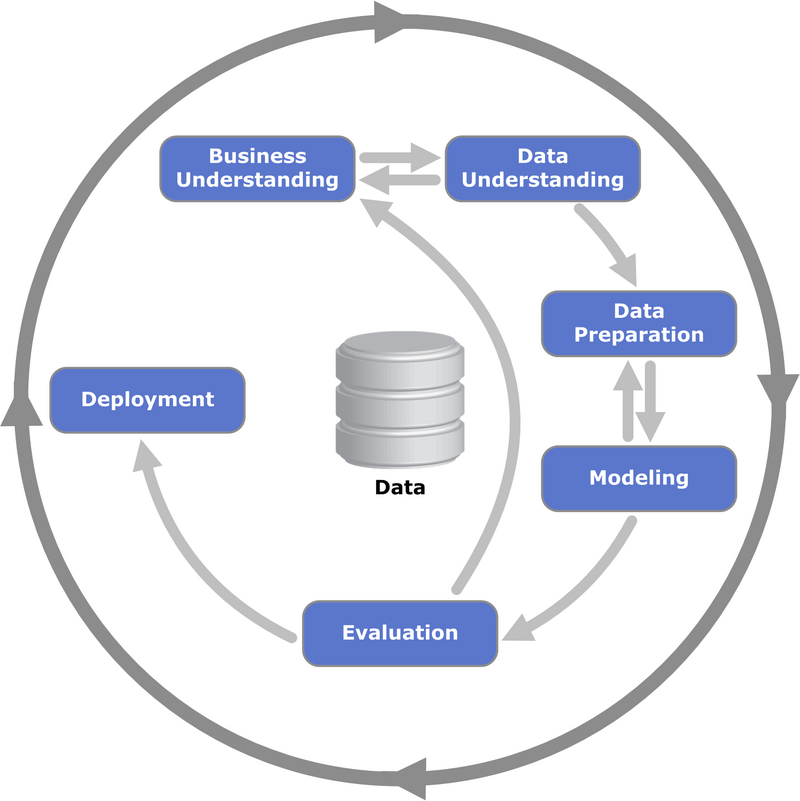
\includegraphics[scale=2.6]{images/CRISP-DM_Process_Diagram.png}}
    \caption{Etapas do processo CRISP-DM. \cite{crispdm}}
    \label{fig:one}
\end{figure}

\subsection{Entendimento do Negócio}
O objetivo foi identificar fatores associados à evasão estudantil em cursos presenciais de bacharelado em computação, utilizando microdados do INEP 2023. Definiu-se a variável alvo \mbox{target\_evadiu} (1 = evadido, 0 = não evadido), permitindo formular o problema como uma tarefa de classificação binária.

\subsection{Entendimento dos Dados}
O conjunto obtido na plataforma PNP foi filtrado para incluir apenas cursos de computação presenciais. Foram exploradas distribuições, tipos de variáveis e tratados valores ausentes; variáveis categóricas foram inspecionadas via tabelas de frequência e associação (Cramér’s V e qui-quadrado), enquanto variáveis numéricas foram analisadas por histogramas, boxplots e correlação de Pearson com a variável alvo.

\subsection{Preparação dos Dados}
As etapas incluíram:

\begin{itemize}
  \item \textbf{Filtragem e limpeza:} remoção de colunas irrelevantes (identificadores, agregados regionais etc.).
  
  \item \textbf{Conversão temporal:} extração de ano, mês e semestre a partir de datas de início e matrícula.
  
  \item \textbf{Engenharia de atributos:} criação de \mbox{Duracao\_Prevista}, \mbox{Tempo\_ate\_Matricula}, \mbox{Mes\_Inicio} e \mbox{Semestre\_Ocorrencia}.
  
  \item \textbf{Pré-processamento:} imputação (\textit{median} para numéricas, \mbox{\textit{most\_frequent}} para categóricas), padronização (StandardScaler) e codificação (OneHotEncoder/OrdinalEncoder) via \\ \mbox{ColumnTransformer}.
  
  \item \textbf{Balanceamento:} uso de SMOTETomek para mitigar desbalanceamento da variável-alvo no conjunto de treino.
\end{itemize}

\subsection{Modelagem}
Foram testados nove algoritmos dentro de um ImbPipeline: Logistic Regression, Decision Tree, Random Forest, SVM (RBF), KNN, Naive Bayes, LDA, QDA e MLP. Cada modelo foi avaliado com divisão estratificada train\_test\_split (70/30).

\subsection{Avaliação}
As métricas calculadas incluíram Accuracy, Precision, Recall, F1-score e ROC-AUC. Após o treino inicial, procedeu-se ao ajuste de limiar de decisão para cada modelo (otimização via curva Precision–Recall) visando maximizar o F1-score. Matrizes de confusão e curvas de desempenho foram geradas para análise comparativa.

\subsection{Interpretação e Importância de Variáveis}
Modelos com atributos interpretáveis tiveram suas importâncias de variáveis ou coeficientes extraídos e ranqueados. As variáveis temporais e institucionais mostraram maior relevância, indicando a influência do tempo até matrícula e a duração prevista sobre a probabilidade de evasão.


\section{Análise Comparativa de Metodologias para Predição de Evasão Estudantil}
O desafio da evasão estudantil é um problema recorrente e complexo, com impactos acadêmicos, sociais e econômicos para as instituições e para os alunos. Diante do volume crescente de dados educacionais, o uso de técnicas de Mineração de Dados (MD) e Aprendizado de Máquina (ML) vem se consolidando como estratégia eficaz para desenvolver modelos preditivos que auxiliem na redução da evasão.

A seguir, apresenta-se uma análise comparativa detalhada entre a metodologia proposta no artigo preliminar (“Previsão da evasão de alunos de cursos de computação no Brasil usando Aprendizado de Máquina”) e os seis artigos de referência.

\newpage

\subsection{Metodologia de Mineração de Dados}

\begin{longtable}{|p{3cm}|p{3.5cm}|p{4.5cm}|p{5cm}|}
    \caption{Comparação de metodologias de Mineração de Dados para predição de evasão estudantil}\\
    \toprule
    \textbf{Artigo} & \textbf{Metodologia de MD Explícita} & \textbf{Fases/Etapas Principais} & \textbf{Alinhamento e Diferenciação} \\
    \midrule
    \endfirsthead
    \toprule
    \textbf{Artigo} & \textbf{Metodologia de MD Explícita} & \textbf{Fases/Etapas Principais} & \textbf{Alinhamento e Diferenciação} \\
    \midrule
    \endhead
    Nosso artigo & CRISP-DM & 1. Coleta; 2. Pré-processamento; 3. Modelagem; 4.Avaliação. & Segue o fluxo clássico de MD (similar ao KDD/CRISP-DM), com foco em múltiplos algoritmos. \\ \hline
    
    Jesus \& Gusmão (2024) & Mapeamento Sistemático da Literatura & 1. Questões; 2. Identificação; 3. Seleção; 4. Síntese. & Caracteriza o estado da arte e destaca lacuna na padronização de atributos. \\ \hline
    
    Jesus (2024) & CRISP-DM & 1. Entendimento; 2. Pre- paração; 3. Modelagem; 4. Avaliação; 5. Implantação. & Adota explicitamente o CRISP-DM e propõe modelo reutilizável com base INEP. \\ \hline
    
    Ramos et al. (2018) & KDD (Knowledge Discovery in Databases) & Pré-processamento; Mineração de Dados; Pós-processamento. & Destaca Análise Fatorial Confirmatória na seleção de variáveis. \\ \hline
    
    Tamada et al. (2019) & Revisão Sistemática da Literatura & Planejamento; Condução; Relatório. & Enfatiza soluções proativas de redução de evasão. \\ \hline
    
    Andrade-Girón et al. (2023) & Revisão Sistemática (PRISMA) & Segue as diretrizes PRISMA. & Avalia desempenho de algoritmos (acurácia, recall, AUC). \\ \hline
    
    Neves (2024) & Framework FICARE & 1. Busca; 2. Construção; 3. Aplicação; 4. Avaliação. & Integra MD, Mineração de Textos e questionários subjetivos. \\
    \bottomrule
\end{longtable}

O presente artigo adota uma metodologia empírica de ML para classificação, em sintonia com a prática observada nos estudos. A escolha do CRISP-DM em \cite{jesus2024mapeamento} e o uso do KDD em \cite{ramos2018comparativo} demonstram o alinhamento com metodologias formais de Descoberta de Conhecimento em Bancos de Dados. O ponto de maior diferenciação é o trabalho de \cite{neves2024ficare}, que eleva o nível da proposta ao criar um framework customizado (FICARE) que inclui a coleta de dados não apenas de sistemas acadêmicos (ERP/AVA) mas também de questionários de escuta ativa (dados subjetivos/textuais).


\newpage
\subsection{Contexto de Dados e Escopo}

\begin{longtable}{|p{3cm}|p{3.5cm}|p{4.5cm}|p{5cm}|}
    \caption{Contexto dos dados e escopo dos estudos comparados}\\
    \toprule
    \textbf{Artigo} & \textbf{Fonte de Dados} & \textbf{Escopo do Estudo} & \textbf{Observações e Características Relevantes} \\
    \midrule
    \endfirsthead
    \toprule
    \textbf{Artigo} & \textbf{Fonte de Dados} & \textbf{Escopo do Estudo} & \textbf{Observações e Características Relevantes} \\
    \midrule
    \endhead
    Nosso artigo & Plataforma Nilo Peçanha (PNP) / Censo da Educação Superior (INEP). & Ensino Superior, cursos de computação na Rede Federal. & Visa generalização nacional. \\ \hline
    
    Jesus \& Gusmão (2024) & Bases bibliográficas diversas. & Ensino superior presencial. & Revelou predominância de estudos no ensino superior e falta de padronização nos conjuntos de atributos utilizados e nas métricas aplicadas para avaliar a evasão. \\ \hline
    
    Jesus (2024) & Censo da Educação Superior (INEP, 2016–2017) & Educação a Distância (EAD) e presencial, instituições públicas e privadas. & Utiliza dados oficiais padronizados e comparáveis entre diferentes instituições. O estudo busca encontrar variáveis universais para modelagem da evasão, com foco em características institucionais e de curso. \\ \hline
    
    Ramos et al. (2018) & Ambiente Virtual de Aprendizagem (AVA) de uma instituição pública & Cursos de graduação na modalidade EAD. & Analisa logs de interação no ambiente virtual (tempo de acesso, atividades realizadas, frequência de participação), relacionando-os ao desempenho acadêmico e evasão. O foco é institucional, limitado a uma única IES. \\ \hline
    
    Tamada et al. (2019) & Diversos ambientes de aprendizagem online (MOOCs e VLEs). & Ensino Superior a distância, cursos massivos online. & Destaca as taxas elevadas de evasão nos MOOCs e a importância da personalização das trilhas de aprendizagem para redução da evasão. Estudo de caráter analítico e comparativo, sem coleta primária de dados. \\ \hline
    
    Andrade-Girón et al. (2023) & Revisão de estudos empíricos sobre evasão. & Ensino Superior (presencial e a distância). & Análise de 43 estudos empíricos. Identifica que o Random Forest é o algoritmo mais frequente e com melhor desempenho médio para detecção de evasão. \\ \hline
    
    Neves (2024) & Ambiente Virtual de Aprendizagem (AVA), Sistema Acadêmico e Questionários de escuta ativa. & Ensino Superior a distância, instituições públicas federais. & Propõe o framework FICARE, que integra dados quantitativos (sistemas institucionais) e qualitativos (questionários) para detecção e mitigação de evasão. Destaca a importância de combinar dados objetivos e subjetivos. \\ 
    \bottomrule
\end{longtable}

O presente estudo faz uso do Censo da Educação Superior do Inep, alinhando-se diretamente com o objetivo de generalização e reutilização de modelos (H2) proposto por \cite{jesus2024mapeamento}. A maioria dos trabalhos focam em dados internos e específicos de uma única IES (\cite{ramos2018comparativo}, \cite{neves2024ficare}) ou em plataformas de larga escala (MOOCs, \cite{tamada2025predicting}). A escolha do Censo Inep (dados governamentais padronizados) na prévia é uma força metodológica para o escopo nacional e para a proposta de criar modelos reutilizáveis.


\subsection{Algoritmos e Métricas de Avaliação}

\begin{longtable}{|p{3cm}|p{3.5cm}|p{4.5cm}|p{5cm}|}
    \caption{Comparativo de algoritmos e métricas}\\
    \toprule
    \textbf{Artigo} & \textbf{Algoritmos de ML Principais} & \textbf{Métricas de Avaliação} & \textbf{Modelo Vencedor/Destaque} \\
    \midrule
    \endfirsthead
    \toprule
    \textbf{Artigo} & \textbf{Algoritmos de ML Principais} & \textbf{Métricas de Avaliação} & \textbf{Modelo Vencedor/Destaque} \\
    \midrule
    \endhead
    Nosso artigo & Regressão Logística (LR), Árvores de Decisão (DT), Random Forest (RF), K-Nearest Neighbors (KNN), Naïve Bayes (NB), Support Vector Machine (SVM), Redes Neurais (MLP). & Acurácia, Precisão, Recall, F1-Score, AUC. & Análise comparativa. \\ \hline
    
    Jesus \& Gusmão (2024) & DT (35), LR (27), SVM (22), RF (25), Redes Neurais (20). & Acurácia, Curva ROC (no mapeamento). & Árvore de Decisão é o mais frequentemente utilizado. \\ \hline
    
    Jesus (2024) & LR, DT, RF, SVM. & VP, VN, FP, FN, Acurácia, Precisão, Recall, Especificidade. & Decision Tree (DT) (Acurácia de 0,979 para EAD Pública). \\ \hline
    
    Ramos et al. (2018) & DT, SVM, NeuralNet, KNN, RegLog. & Precisão, Recall, Acurácia, AUC. & Regressão Logística (Acurácia de 0,894; Recall mais alto: 0,617). \\ \hline
    
    Tamada et al. (2019) & LR, SVM, DT, DL, RNN/LSTM (mais usados: LR e SVM). & Acurácia (ACC). & Varia (DL, RF, SVM, RNN/LSTM), com SVM/Deep Learning apresentando alta acurácia (99,64\%). \\ \hline
    
    Andrade-Girón et al. (2023) & Random Forest (RF) (21,73\%), LR, DT, SVM, Redes Neurais (39,13\%). & Acurácia, Sensibilidade/Recall, Especificidade, AUC. & Random Forest (RF) (Acurácia de 99\%). \\ \hline
    
    Neves (2024) & SVM (com diferentes kernels), LR, DT, RF, Redes Neurais. & VP, VN, FP, FN, Acurácia, Precisão, Recall, Especificidade, G-means, F-measure, Índice Kappa. & SVM com kernel RBF (Acurácia de 93,22\%; G-means de 87,65\% para Reprovação). \\ 
    \bottomrule
\end{longtable}

O presente trabalho propõe a testagem de um conjunto abrangente de algoritmos de classificação supervisionada, refletindo a diversidade observada na literatura (\cite{jesus2024mapeamento}, \cite{tamada2025predicting}).

Embora a Decision Tree (DT) seja o algoritmo mais frequentemente utilizado (\cite{jesus2024mapeamento}), o Random Forest (RF) emerge como o mais robusto em algumas revisões (\cite{andradegiron2023predicting}), e a Regressão Logística (LR) se destaca pela interpretabilidade (\cite{ramos2018comparativo}) e alta precisão em alguns cenários de EAD.

Todos os trabalhos usam as métricas básicas (Acurácia, Precisão, Recall). No entanto, a proposta de \cite{neves2024ficare} de incluir F-measure (média harmônica de precisão e recall) e G-means (média geométrica de recall e especificidade) é crucial para lidar com bases de dados desbalanceadas (onde os casos de evasão/reprovação são minoritários), garantindo que o modelo não seja enviesado para a classe majoritária (não-evadidos/aprovados). A inclusão dessas métricas na prévia é um ponto forte para a avaliação científica.


\newpage
\subsection{Variáveis Mais Influentes}

A escolha dos atributos é um passo crítico do processo KDD/CRISP-DM.

\begin{longtable}{|p{3cm}|p{5.5cm}|p{7cm}|}
    \caption{Análise de variáveis e sua relevância}\\
    \toprule
    \textbf{Artigo} & \textbf{Variáveis Mais Relevantes/ Foco} & \textbf{Relevância para o Artigo Preliminar} \\
    \midrule
    \endfirsthead
    \toprule
    \textbf{Artigo} & \textbf{Variáveis Mais Relevantes / Foco} & \textbf{Relevância para o Artigo Preliminar} \\
    \midrule
    \endhead
    Nosso artigo & Variáveis demográficas, socioeconômicas e acadêmicas do Censo Inep. & Totalmente alinhado, pois o Censo do Inep é a fonte declarada e possui essa taxonomia de dados. \\ \hline
    
    Jesus (2024) & IN\_CONCLUINTE (aluno no último período) e CO\_ALUNO\_SITUACAO (situação de vínculo). & Crucial: Estas variáveis do Censo (INEP) são identificadas como as mais importantes em todos os cenários (EAD/Presencial, Público/Privado). A prévia deve focar na extração e análise dessas features do Censo. \\ \hline
    
    Ramos et al. (2018) & Métricas de interação no AVA (acessos por turno, tempo médio, posts, mensagens enviadas/recebidas). & Complementar: O foco são os dados de comportamento e log do AVA, que são difíceis de obter de forma padronizada (Censo). \\ \hline
    
    Tamada et al. (2019) & Clickstream, participação em fóruns, notas de quizzes. & Complementar (Dados de Log): Os logs de acesso, como no Censo Inep, não têm a granularidade de clickstream (pausa, rewind), mas sim de situação de vínculo/matrícula. \\ \hline
    
    Neves (2024) & Dados de sistemas (AVA/WebGiz), mas principalmente de questionários (Perfil do Ingressante: gênero, renda, experiência com EaD). & Complementar: Neves sugere que o dado de questionário (auto-declaração) é um complemento valioso para o dado de sistema (registro acadêmico), possível recomendação para futuras extensões do presente estudo \\ 
    \bottomrule
\end{longtable}

Diferente da maioria dos estudos de caso (\cite{ramos2018comparativo}, \cite{neves2024ficare}), o uso do Censo Inep em um recorte de cursos de Computação (Ensino Superior) permite a criação e avaliação de um modelo preditivo com base de dados padronizada em nível nacional (como proposto por \cite{jesus2024mapeamento}), mitigando o problema da não-reutilização de modelos entre diferentes IES (H2 verdadeira em \cite{jesus2024mapeamento}).

A inclusão de métricas como F1-Score e AUC no presente trabalho o posiciona em um nível de avaliação robusta, necessário para bases desbalanceadas, superando o uso exclusivo de métricas menos informativas (como apenas Acurácia) que podem mascarar o baixo desempenho na classe minoritária (evadidos).

O conjunto de sete algoritmos testados é mais amplo do que a maioria dos trabalhos de comparação, garantindo que o modelo "vencedor" seja o mais robusto.


\subsection{Conclusão da Análise Comparativa}

\begin{longtable}{|p{7cm}|p{8cm}|}
    \caption{Síntese comparativa final}\\
    \toprule
    \textbf{Ponto Forte do presente trabalho} & \textbf{Comparativo com a Literatura} \\
    \midrule
    \endfirsthead
    \toprule
    \textbf{Ponto Forte do presente trabalho} & \textbf{Comparativo com a Literatura} \\
    \midrule
    \endhead
    Uso da Base Inep (Censo da Educação Superior) & Alinhado com a proposta de \cite{jesus2024dissertacao} para reutilização e padronização nacional, e se diferencia dos estudos de caso localizados (\cite{ramos2018comparativo}) ou de plataformas específicas (\cite{tamada2025predicting}). \\ \hline

    Metodologia de ML Abrangente & O teste de sete algoritmos supervisionados é um procedimento robusto, apoiado pelo mapeamento de \cite{jesus2024mapeamento} e pela busca de algoritmos de melhor desempenho (\cite{andradegiron2023predicting}). \\ \hline
    
    Métricas de Avaliação Robustas (F1-Score, AUC) & Essencial para lidar com o desbalanceamento de classes, metodologia apoiada pela análise de \cite{neves2024ficare}. \\
    \bottomrule
\end{longtable}

O atual trabalho contribui para a literatura preenchendo a lacuna de um modelo preditivo nacionalmente padronizado para cursos de computação. A identificação das métricas mais relevantes (como as já destacadas por \cite{jesus2024mapeamento}) dentro do contexto dos cursos de computação será o principal resultado prático, orientando intervenções institucionais.


\section{Engenharia de Atributos e Exploração Inicial}

\subsection{Engenharia de Atributos}
O processo de preparação envolveu a transformação sistemática dos microdados da Plataforma Nilo Peçanha (PNP) em um conjunto estruturado e analiticamente consistente.  
Inicialmente, foi criada a variável alvo \mbox{target\_evadiu}, codificando a evasão de forma binária (1 = evadido, 0 = não evadido), a partir da coluna Categoria da Situação. Essa etapa converteu informações textuais sobre situação acadêmica em formato adequado à modelagem supervisionada.

Posteriormente, aplicaram-se filtros para restringir o escopo aos cursos presenciais de bacharelado exclusivamente da área de Computação, contemplando: Análise e Desenvolvimento de Sistemas, Ciência da Computação, Computação, Engenharia de Computação, Engenharia de Telecomunicações, Gestão da Tecnologia da Informação, Informática, Jogos Digitais, Redes de Computadores, Sistemas de Informação, Sistemas para Internet, Telemática e Agrocomputação.  
Essa filtragem assegura a homogeneidade do domínio e elimina registros de cursos não correlatos.

Variáveis redundantes, administrativas ou descritivas foram removidas, preservando apenas atributos relevantes ao perfil discente e à trajetória acadêmica. As variáveis temporais (Data de Início do Ciclo, Data de Fim Previsto do Ciclo e Data de Ocorrência da Matrícula) foram convertidas para o tipo datetime e utilizadas para gerar novos atributos derivados:

\begin{itemize}
    \item \textbf{Duração Prevista}: diferença em dias entre as datas de início e término previstas do ciclo;
    \item \textbf{Tempo até Matrícula}: intervalo entre o início do curso e a data efetiva da matrícula;
    \item \textbf{Mês de Início} e \textbf{Semestre de Ocorrência}: atributos categóricos derivados das datas, refletindo sazonalidade e períodos de ingresso;
    \item \textbf{Ano-Mês de Ocorrência}: representação temporal útil para análise agregada e variações anuais.
\end{itemize}

Essas variáveis capturam dimensões cronológicas e institucionais que influenciam o risco de evasão, enriquecendo o espaço de atributos e permitindo modelagem mais interpretável. Após a derivação, as colunas originais de data foram removidas para evitar redundância e colinearidade.

\subsection{Exploração Inicial}

Na fase exploratória, as variáveis numéricas foram inspecionadas individualmente por meio de histogramas e boxplots, identificando padrões de distribuição, assimetrias e outliers.

\begin{figure}[H]\centering
    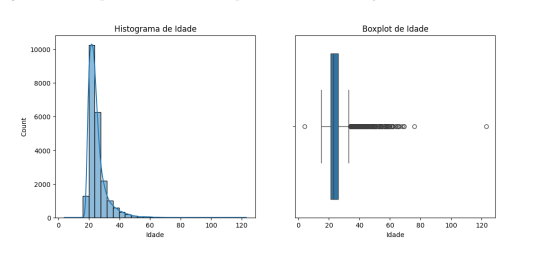
\includegraphics[width=1\textwidth]{images/descritivo-idade.png}
    \caption{Distribuição e boxplot da variável Idade.}
    \label{fig:idade}
\end{figure}

\begin{figure}[H]\centering
	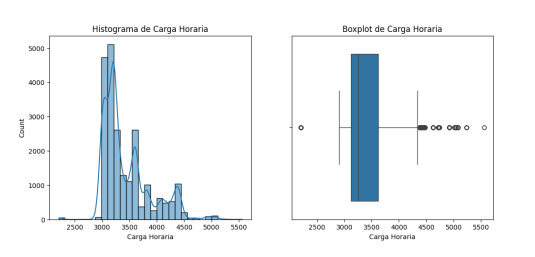
\includegraphics[width=1\textwidth]{images/descritivo-carga-horaria.png}
	\caption{Distribuição e boxplot da variável Carga Horária.}
	\label{fig:carga-horaria}
\end{figure}

\begin{figure}[H]\centering
	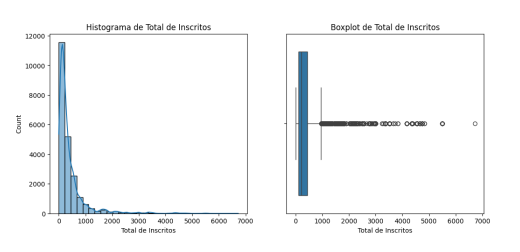
\includegraphics[width=1\textwidth]{images/descritivo-inscritos.png}
	\caption{Distribuição e boxplot da variável Total de Inscritos.}
	\label{fig:total-inscritos}
\end{figure}

As análises evidenciam distribuições assimétricas com concentração dos valores em faixas específicas e presença de outliers representando casos atípicos. A idade apresenta forte concentração entre 18 e 25 anos, enquanto a carga horária e o número de inscritos exibem maior dispersão entre instituições.

A seguir, avaliaram-se as correlações lineares entre variáveis numéricas e a variável alvo (\mbox{target\_evadiu}), além das correlações entre as próprias variáveis numéricas:

\begin{figure}[H]\centering
	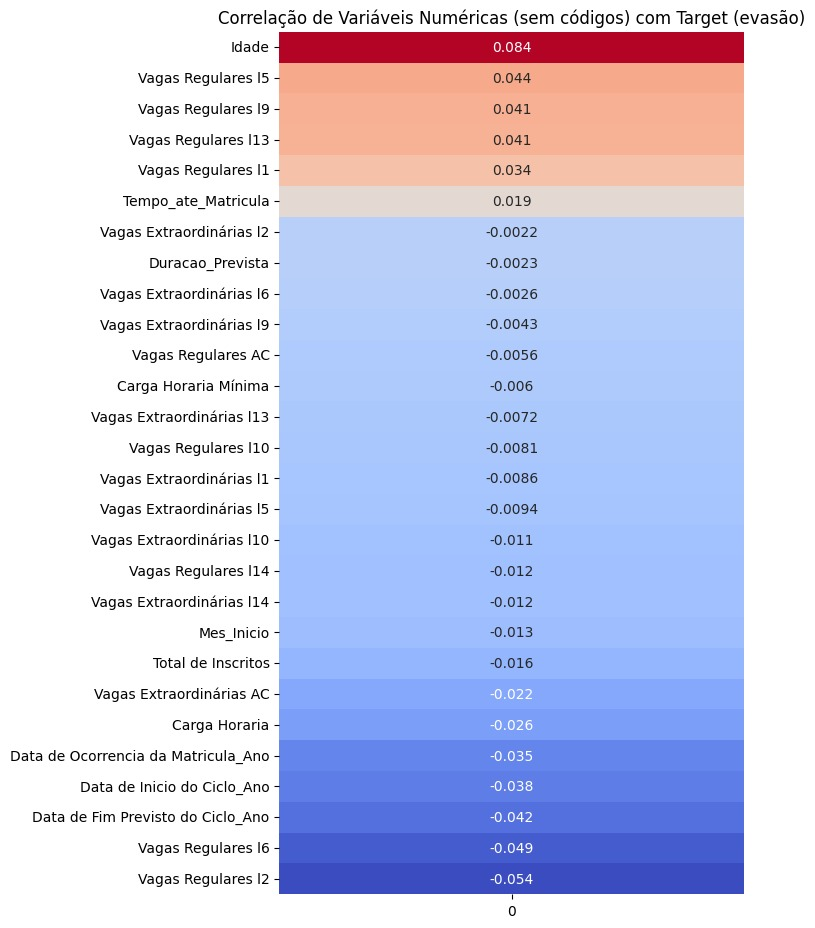
\includegraphics[width=1\textwidth]{images/correlacao_variaveis_num_com_target.jpeg}
	\caption{Correlação entre variáveis numéricas e a variável alvo \mbox{(target\_evadiu)}.}
	\label{fig:corr-num-target}
\end{figure}

\begin{figure}[H]\centering
	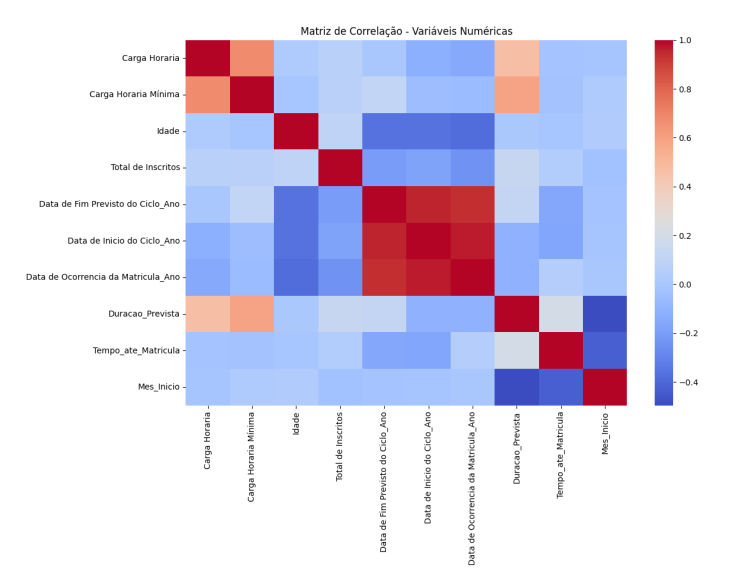
\includegraphics[width=1\textwidth]{images/matriz-corr.png}
	\caption{Matriz geral de correlação entre variáveis numéricas.}
	\label{fig:corr-num-geral}
\end{figure}


\subsection{Análise das Variáveis Categóricas}

Investigou-se as variáveis categóricas e sua relação com a evasão, utilizando o teste qui-quadrado e o coeficiente de associação Cramér’s V. Para cada atributo, são apresentados os resultados tabulares e os respectivos histogramas comparativos com a variável alvo.

\begin{table}[H]
	\centering
	\caption{Associação entre Turno e evasão.}
	\label{tab:cat-turno}
	\begin{tabular}{lcc}
		\toprule
		\textbf{Turno} & \textbf{Não evadido (0)} & \textbf{Evadido (1)} \\
		\midrule
		Integral & 0.866557 & 0.133443 \\
		Matutino & 0.777497 & 0.222503 \\
		Noturno & 0.860302 & 0.139698 \\
		Vespertino & 0.906754 & 0.093246 \\
		\bottomrule
	\end{tabular}
\end{table}

\begin{figure}[H]\centering
	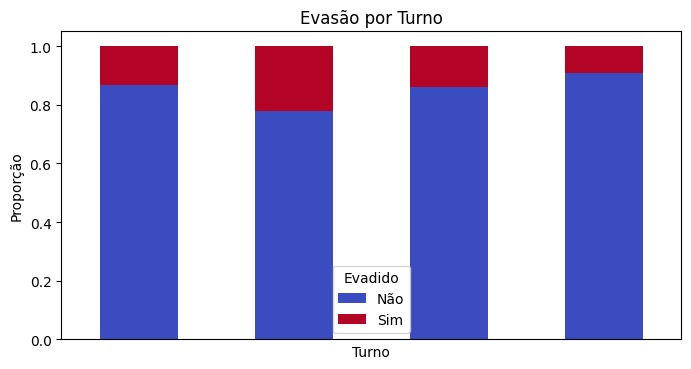
\includegraphics[width=0.8\textwidth]{images/evasao-turno.jpeg}
	\caption{Distribuição de evasão por Turno.}
	\label{fig:cat-turno-hist}
\end{figure}

\begin{table}[H]
	\centering
	\caption{Associação entre Região e evasão.}
	\label{tab:cat-regiao}
	\begin{tabular}{lcc}
		\toprule
		\textbf{Região} & \textbf{Não evadido (0)} & \textbf{Evadido (1)} \\
		\midrule
		Centro-Oeste & 0.874612 & 0.125388 \\
		Nordeste & 0.881981 & 0.118019 \\
		Norte & 0.911411 & 0.088589 \\
		Sudeste & 0.874414 & 0.125586 \\
		Sul & 0.726864 & 0.273136 \\
		\bottomrule
	\end{tabular}
\end{table}

\begin{figure}[H]\centering
	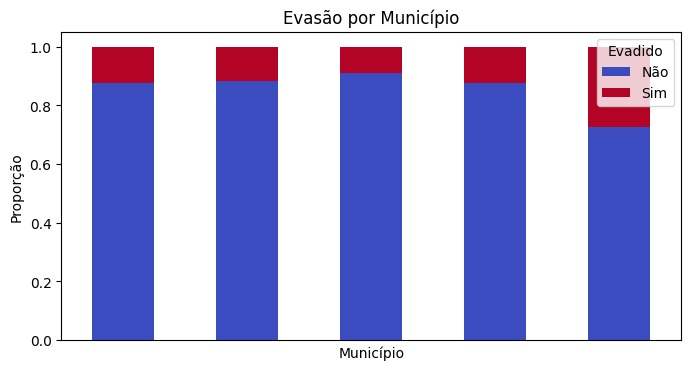
\includegraphics[width=0.8\textwidth]{images/evasao-municipio.jpeg}
	\caption{Distribuição de evasão por Região.}
	\label{fig:cat-regiao-hist}
\end{figure}

\begin{table}[H]
	\centering
	\caption{Associação entre Faixa Etária e evasão.}
	\label{tab:cat-faixa}
	\begin{tabular}{lcc}
		\toprule
		\textbf{Faixa Etária} & \textbf{Não evadido (0)} & \textbf{Evadido (1)} \\
		\midrule
		15 a 19 anos & 0.923018 & 0.076982 \\
		20 a 24 anos & 0.886965 & 0.113035 \\
		25 a 29 anos & 0.823562 & 0.176438 \\
		30 a 34 anos & 0.768817 & 0.231183 \\
		35 a 39 anos & 0.750000 & 0.250000 \\
		40 a 44 anos & 0.757732 & 0.242268 \\
		45 a 49 anos & 0.821782 & 0.178218 \\
		50 a 54 anos & 0.722892 & 0.277108 \\
		55 a 59 anos & 0.654545 & 0.345455 \\
		Maior de 60 anos & 0.657895 & 0.342105 \\
		\bottomrule
	\end{tabular}
\end{table}

\begin{figure}[H]\centering
	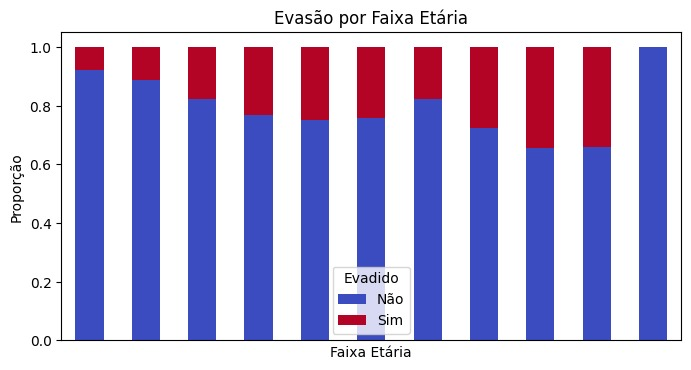
\includegraphics[width=0.8\textwidth]{images/evasao-faixa-etara.jpeg}
	\caption{Distribuição de evasão por Faixa Etária.}
	\label{fig:cat-faixa-hist}
\end{figure}

\begin{table}[H]
	\centering
	\caption{Associação entre Curso e evasão.}
	\label{tab:cat-curso}
	\begin{tabular}{lcc}
		\toprule
		\textbf{Nome de Curso} & \textbf{Não evadido (0)} & \textbf{Evadido (1)} \\
		\midrule
		Análise e Desenvolvimento de Sistemas & 0.990909 & 0.009091 \\
		Ciência da Computação & 0.836382 & 0.163618 \\
		Engenharia de Computação & 0.884044 & 0.115956 \\
		Engenharia de Telecomunicações & 0.818642 & 0.181358 \\
		Informática & 0.835821 & 0.164179 \\
		Sistemas de Informação & 0.857127 & 0.142873 \\
		\bottomrule
	\end{tabular}
\end{table}

\begin{figure}[H]\centering
	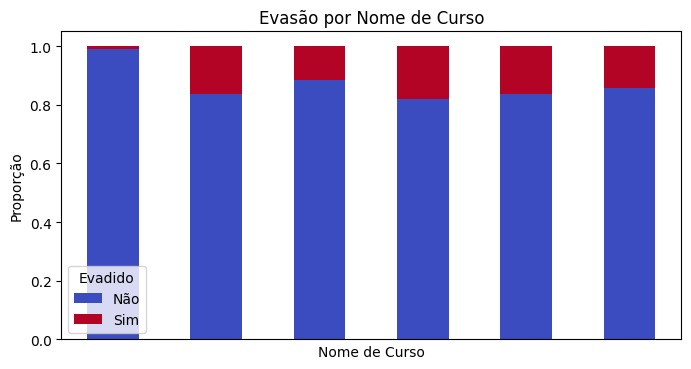
\includegraphics[width=0.8\textwidth]{images/evasao-nome-curso.jpeg}
	\caption{Distribuição de evasão por Curso.}
	\label{fig:cat-curso-hist}
\end{figure}

As análises categóricas revelam padrões distintos de evasão entre regiões, turnos e cursos, indicando que fatores institucionais e contextuais exercem influência significativa sobre o comportamento de permanência dos estudantes.


\section{Modelagem e Avaliação}

\subsection{Visão geral do processo}

Aplicamos um fluxo padrão de aprendizado supervisionado: (i) preparação dos dados com imputação, padronização e codificação; (ii) balanceamento do conjunto de treino; (iii) treinamento de múltiplos classificadores; (iv) avaliação no conjunto de teste. O foco foi comparar desempenho preditivo em vez de detalhar hiperparâmetros. Todas as métricas foram calculadas com limiar de decisão padrão ($0{,}5$), salvo indicação em contrário.

\subsection{Procedimento de avaliação}
A avaliação priorizou F1-score, Recall e ROC-AUC. As matrizes de confusão são apresentada aos pares.

\begin{figure}[H]\centering
    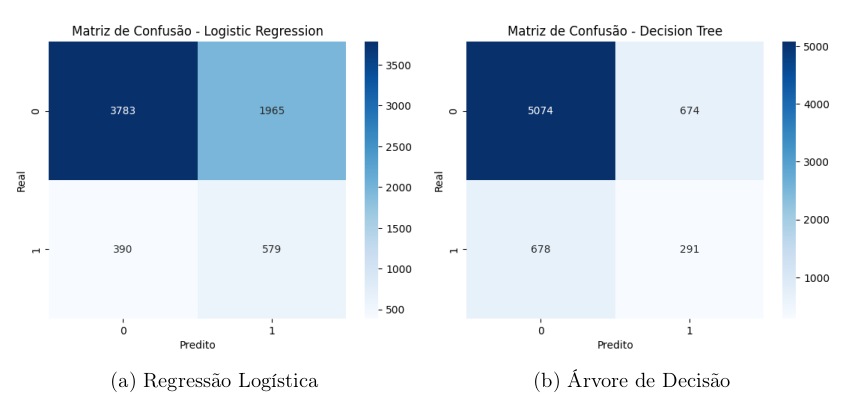
\includegraphics[width=1\textwidth]{images/matrizes-confusao-log-dec.png}
    \caption{Matrizes de confusão para Regressão Logística e Árvore de Decisão. Threshold = 0{,}5.}
    \label{fig:cms-a}
\end{figure}

\begin{figure}[H]\centering
    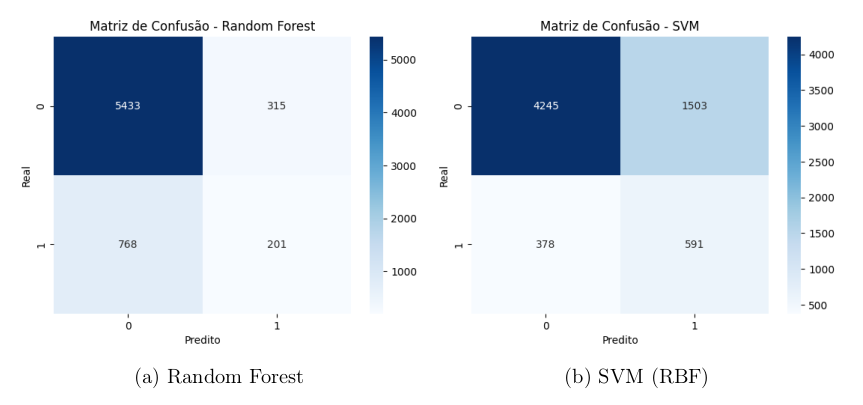
\includegraphics[width=1\textwidth]{images/matrizes-confusao-for-svm.png}
    \caption{Matrizes de confusão para Random Forest e SVM. Threshold = 0{,}5.}
    \label{fig:cms-b}
\end{figure}

\begin{figure}[H]\centering
    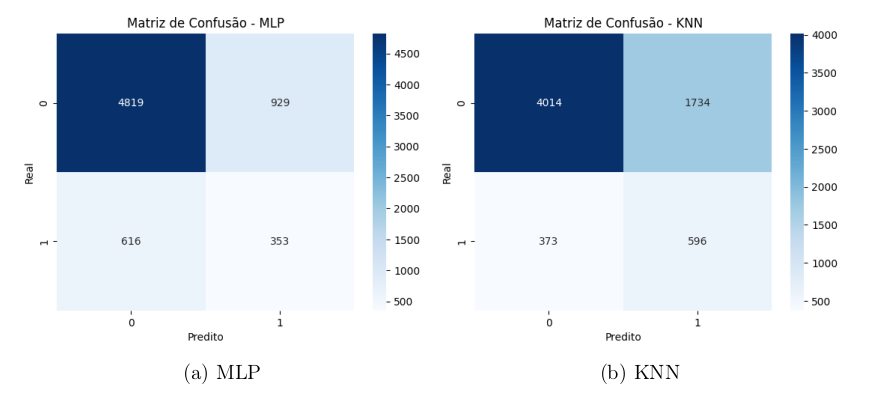
\includegraphics[width=1\textwidth]{images/matrizes-confusao-mlp-knn.png}
    \caption{Matrizes de confusão para MLP e kNN. Threshold = 0{,}5.}
    \label{fig:cms-c}
\end{figure}

\begin{figure}[H]\centering
    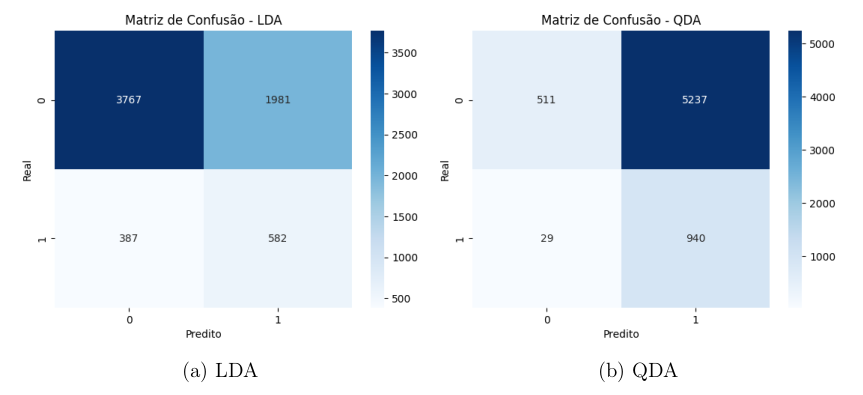
\includegraphics[width=1\textwidth]{images/matrizes-confusao-lda-qda.png}
    \caption{Matrizes de confusão para LDA e QDA. Threshold = 0{,}5.}
    \label{fig:cms-d}
\end{figure}

\begin{figure}[htbp]\centering
	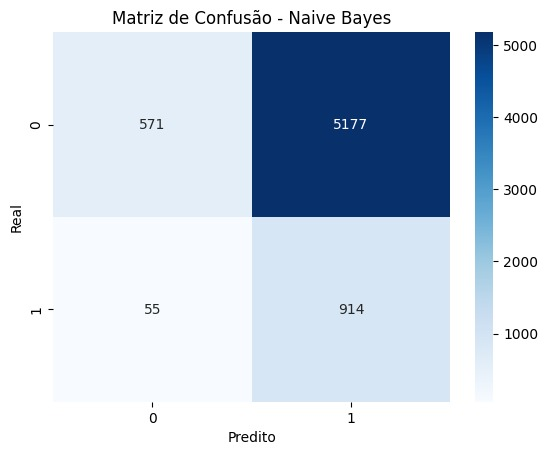
\includegraphics[width=0.6\textwidth]{images/matriz-confusao-naive-bayes.jpeg}
	\caption{Matriz de confusão para Naive Bayes. Threshold = 0{,}5.}
	\label{fig:cms-nb}
\end{figure}


\subsection{Comparação global dos modelos}

\begin{table}[H]
	\centering
	\caption{Comparação de desempenho entre modelos com threshold padrão (0,5).}
	\label{tab:comparacao-global}
	\begin{tabular}{lrrrrr}
	\toprule
	\textbf{Modelo} & \textbf{Accuracy} & \textbf{Precision} & \textbf{Recall} & \textbf{F1-score} & \textbf{ROC-AUC} \\
	\midrule
	SVM                  & 0.719964 & 0.282235 & 0.609907 & 0.385896 & 0.734610 \\
	Random Forest        & 0.838767 & 0.389535 & 0.207430 & 0.270707 & 0.710035 \\
	KNN                  & 0.686318 & 0.255794 & 0.615067 & 0.361322 & 0.706743 \\
	Logistic Regression  & 0.649397 & 0.227594 & 0.597523 & 0.329633 & 0.679301 \\
	LDA                  & 0.647462 & 0.227078 & 0.600619 & 0.329558 & 0.678253 \\
	MLP                  & 0.769987 & 0.275351 & 0.364293 & 0.313638 & 0.668567 \\
	Decision Tree        & 0.798720 & 0.301554 & 0.300310 & 0.300931 & 0.594230 \\
	Naive Bayes          & 0.221081 & 0.150057 & 0.943240 & 0.258924 & 0.588279 \\
	QDA                  & 0.216019 & 0.152177 & 0.970072 & 0.263084 & 0.549362 \\
	\bottomrule
	\end{tabular}
\end{table}


\subsection{Importância de variáveis e interpretabilidade}

Para modelos com explicabilidade direta, reportamos as 20 variáveis mais relevantes. As importâncias refletem diferentes noções de influência: impureza média reduzida em árvores/ensembles e coeficientes em modelos lineares.

\begin{figure}[H]\centering
	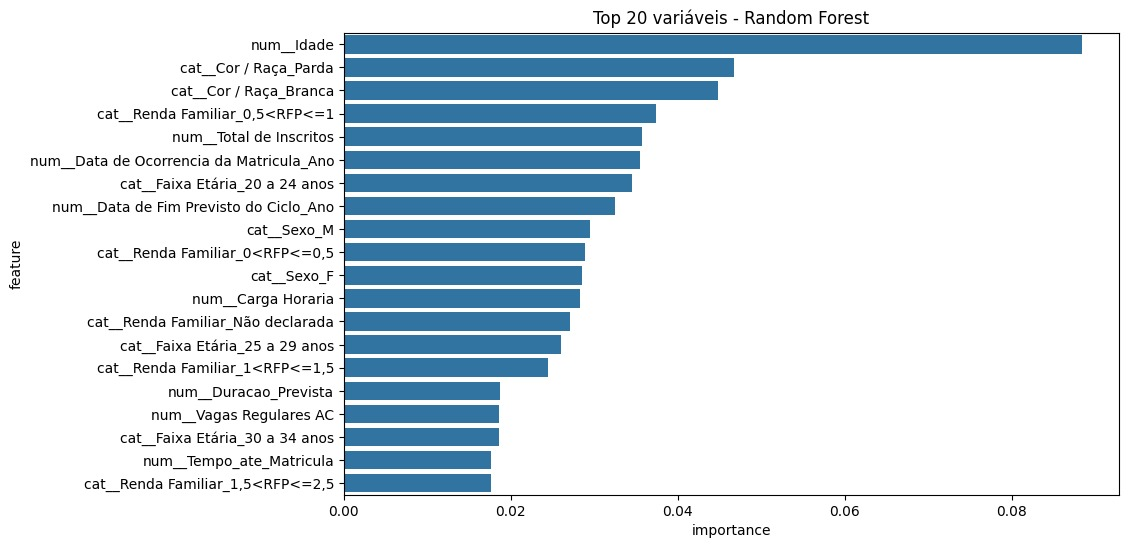
\includegraphics[width=1\textwidth]{images/top20-random-forest.jpeg}
	\caption{Random Forest: 20 variáveis mais importantes.}
	\label{fig:feat-rf}
\end{figure}

\begin{figure}[H]\centering
    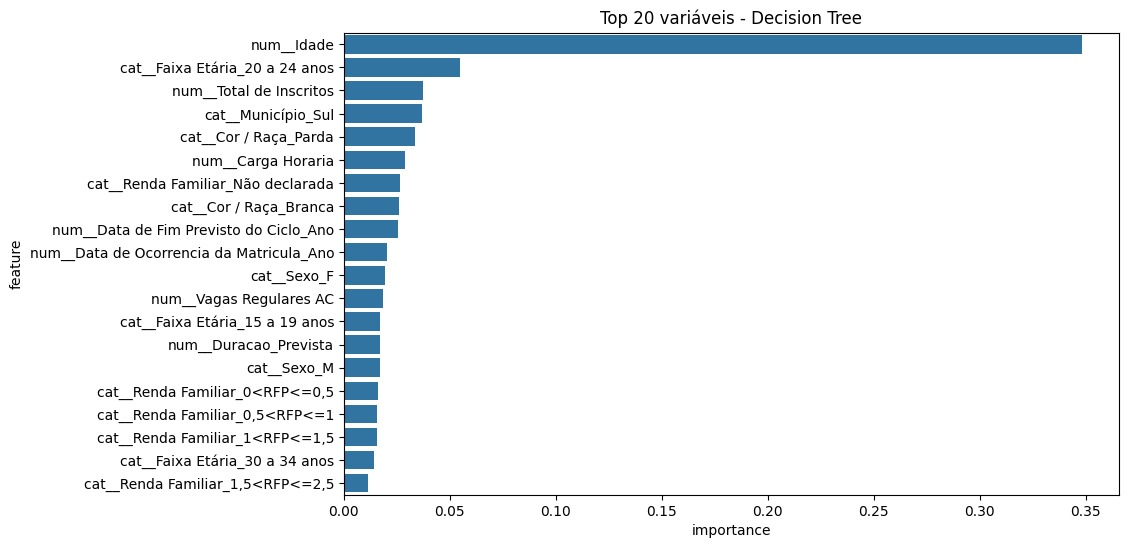
\includegraphics[width=1\textwidth]{images/top20-decision-tree.jpeg}
    \caption{Árvore de Decisão: 20 variáveis mais importantes.}
    \label{fig:feat-dt}
\end{figure}

\begin{figure}[H]\centering
    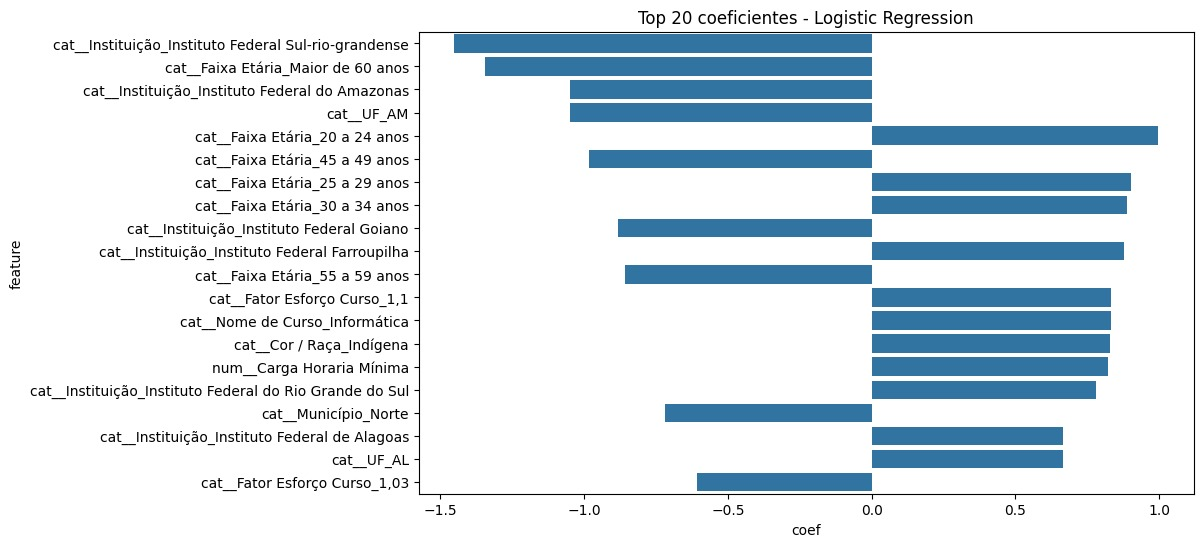
\includegraphics[width=1\textwidth]{images/top20-regr-log.jpeg}
    \caption{Regressão Logística: 20 coeficientes de maior magnitude.}
    \label{fig:feat-lr}
\end{figure}

\begin{figure}[H]\centering
    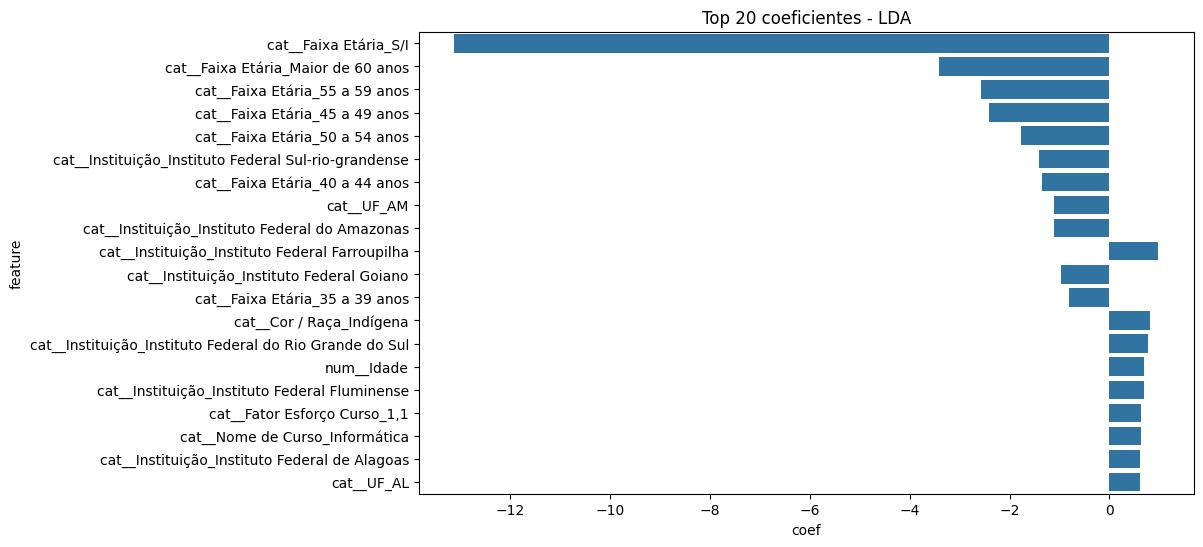
\includegraphics[width=1\textwidth]{images/top20-lda.jpeg}
    \caption{LDA: 20 coeficientes de maior magnitude.}
    \label{fig:feat-lda}
\end{figure}

\newpage
\section{Resultados e Discussão}

\subsection{Desempenho global dos modelos}

A Tabela 10 resume o desempenho dos modelos. O SVM apresentou o melhor F1-score (0,386) e ROC-AUC mais alto (0,735), indicando melhor compromisso entre precisão e sensibilidade. A Random Forest obteve a maior accuracy (0,839), porém com recall baixo (0,207), refletindo postura conservadora na detecção de evadidos. O KNN alcançou recall elevado (0,615) com precision modesta. Naive Bayes e QDA exibiram recall muito alto, porém com queda acentuada em accuracy e F1, sugerindo viés para a classe positiva. Esses achados reforçam que, em bases desbalanceadas, a escolha do limiar e a métrica de avaliação são decisivas.

\begin{table}[H]
	\centering
	\caption{Comparação de desempenho entre modelos com threshold padrão (0,5).}
	\label{tab:comparacao-global}
	\begin{tabular}{lrrrrr}
	\toprule
	M\textbf{odelo} & \textbf{Accuracy} & \textbf{Precision} & \textbf{Recall} & \textbf{F1-score} & \textbf{ROC-AUC} \\
	\midrule
	SVM                  & 0.719964 & 0.282235 & 0.609907 & 0.385896 & 0.734610 \\
	Random Forest        & 0.838767 & 0.389535 & 0.207430 & 0.270707 & 0.710035 \\
	KNN                  & 0.686318 & 0.255794 & 0.615067 & 0.361322 & 0.706743 \\
	Logistic Regression  & 0.649397 & 0.227594 & 0.597523 & 0.329633 & 0.679301 \\
	LDA                  & 0.647462 & 0.227078 & 0.600619 & 0.329558 & 0.678253 \\
	MLP                  & 0.769987 & 0.275351 & 0.364293 & 0.313638 & 0.668567 \\
	Decision Tree        & 0.798720 & 0.301554 & 0.300310 & 0.300931 & 0.594230 \\
	Naive Bayes          & 0.221081 & 0.150057 & 0.943240 & 0.258924 & 0.588279 \\
	QDA                  & 0.216019 & 0.152177 & 0.970072 & 0.263084 & 0.549362 \\
	\bottomrule
	\end{tabular}
\end{table}


\subsection{Matrizes de confusão e erros típicos}

As matrizes da Figura~\ref{fig:cm-grid} mostram os trade-offs. O SVM reduz falsos negativos frente a modelos lineares, à custa de mais falsos positivos. A Random Forest minimiza falsos positivos, mas perde sensibilidade. NB e QDA concentram predições na classe positiva, inviabilizando uso prático.

\begin{figure}[H]\centering
    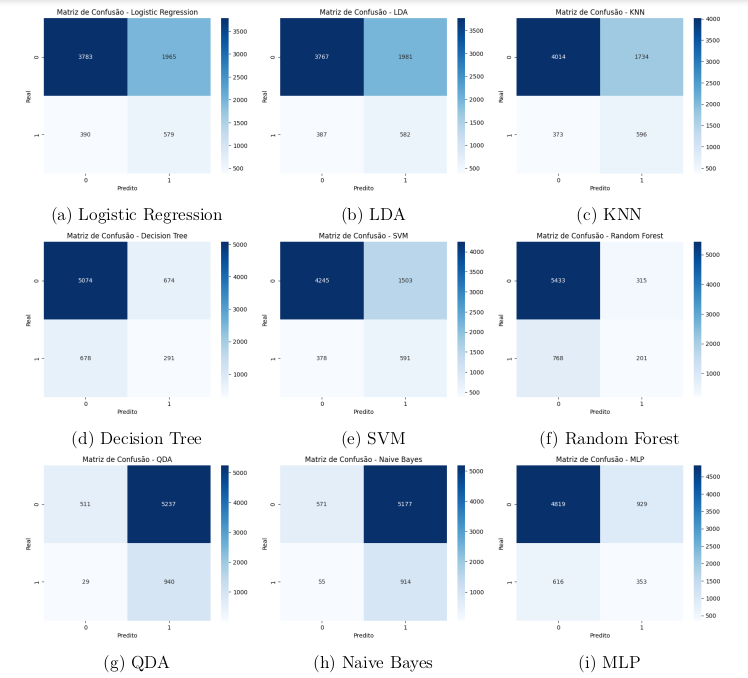
\includegraphics[width=1\textwidth]{images/todas-matrizes.png}
    \caption{Matrizes de confusão no conjunto de teste.}
    \label{fig:cm-grid}
\end{figure}

\subsection{Importância e sinais das variáveis}

As Figuras~\ref{fig:feat-lr} e~\ref{fig:feat-lda} mostram os coeficientes dos modelos lineares. Observa-se efeito etário não linear: aumento de risco em 20–24 anos e nova elevação em faixas acima de 45 anos. Indicadores institucionais e regionais também aparecem com peso. Características demográficas específicas (p. ex.: cor/raça e sexo) e variáveis acadêmico-administrativas (carga horária mínima) têm associação relevante com a evasão.

Para modelos baseados em árvores, as Figuras~\ref{fig:feat-rf} e~\ref{fig:feat-dt} indicam Idade como variável mais importante, seguida de renda familiar (faixas até 1 RFP e não declarada), cor/raça, sexo e variáveis temporais (datas de ocorrência/encerramento do ciclo, duração prevista e tempo até matrícula). Itens de contexto competitivo (total de inscritos e vagas regulares) também contribuem, sugerindo que pressão por vagas e perfis discente-institucionais afetam a permanência. Esses achados são coerentes com a literatura sobre preditores demográficos e acadêmicos.


\subsection{Implicações práticas e síntese}

Objetivando um modelo para alerta precoce. Se a prioridade é sensibilidade, o SVM é candidato inicial. Ajuste de limiar ou calibração pode elevar recall mantendo precisão aceitável.

Se o objetivo é um modelo para decisão conservadora. Quando o custo de falso positivo é alto, a Random Forest favorece maior precisão/acurácia, mesmo com recall menor.

Os fatores-alvo identificados para intervenção foram: Idade, faixas de renda familiar baixa/não declarada, cor/raça, sexo, indicadores temporais do percurso e pressão por vagas. Todos citados aparecem de maneira consistente nos modelos. Políticas de permanência devem considerar apoio financeiro, flexibilidade acadêmica para perfis mais vulneráveis e monitoramento temporal das trajetórias.

Como conclusão, os resultados apontam para um pipeline robusto e reprodutível. SVM e Random Forest lideram em desempenho sob objetivos distintos; variáveis demográficas, socioeconômicas e temporais são determinantes. A adoção institucional deve combinar escolha de modelo ao custo-erro e ações focalizadas sobre os fatores identificados.

\section{Conclusões e Trabalhos Futuros}

A aplicação de modelos preditivos à base de microdados de matrículas demonstra que é possível antecipar casos de evasão com desempenho satisfatório, especialmente quando se adotam processos cuidadosos de engenharia de atributos e balanceamento. Modelos de ensemble, como Random Forest, destacaram-se pela robustez frente a variáveis heterogêneas. Para trabalhos futuros, sugerimos: (i) incorporar informações socioeconômicas individuais, (ii) explorar modelos temporais que considerem sequências de matrículas ao longo dos anos e (iii) integrar indicadores de engajamento em ambientes virtuais, em linha com tendências identificadas na literatura.

Como desdobramentos práticos, recomenda-se que instituições desenvolvam painéis de monitoramento que combinem métricas quantitativas e alertas qualitativos. A adoção de equipes multidisciplinares, com participação de analistas de dados, pedagogos e assistentes sociais, pode acelerar a tradução dos insights em planos de ação. Investir em formação docente para uso de dados educacionais também se revela estratégico, permitindo que cada curso identifique rapidamente mudanças de padrão e acione intervenções personalizadas.


\iffalse
    \cite{tamada2025predicting}
    \cite{jesus2024mapeamento}
    \cite{jesus2024dissertacao}
    \cite{neves2024ficare}
    \cite{andradegiron2023predicting}
    \cite{ramos2018comparativo}
\fi





















\iffalse % Usado para que o compilador ignore.
         % Essencialmente comentar este trecho
    \section*{Acknowledgements}
    %Place the acknowledgements only in the final version of the manuscript, after acceptance. They should be placed before the references section without numbering.
    Our special thanks to Rafael Bohrer Ávila, Matheus Segalotto and Bruno Fagundes da Silva for their help with this latex template. 
\fi






\newpage
\printbibliography
%See the guidelines for metadata and references:
%https://sol.sbc.org.br/journals/index.php/rbie/libraryFiles/downloadPublic/71


\iffalse % Usado para que o compilador ignore.
         % Essencialmente comentar este trecho
     \section*{Appendix 1}
    \label{apendice1}
    
    If any, the appendix should appear directly after the references without numbering, and not on a new page.
    
    \begin{enumerate}
        \item[A] When the reference has a Link
        \begin{itemize}
            \item Make a clickable link on the respective URL (if you are using MS-Word, use the tool Insert Hyperlink, informing the URL).
        \end{itemize}
        \item[B] Allow readers to search for the reference on Google Scholar
        \begin{itemize}
            \item Copy the title of the reference and put in between ``\%22'', including the ``+'' character between each word: http://scholar.google.com/scholar?q=\%22PASTE+TITLE+\\HERE\%22\&hl=en\&lr=\&btnG=Search
            \item If it is a common title, you may add the author, such as in: \\http://scholar.google.com/ scholar?q=PASTE+AUTHOR+HERE+\%22PASTE+TITLE\\+HERE\%22\&hl=en\&lr=\&btnG=Search
            \item Or you may use the publication year (YEAR) to restrict the results, such as in:\\ http://scholar.google.com/scholar?
            q=PASTE+AUTHOR+HERE+\%22PASTE+TITLE\\+HERE\%22\&hl=en\&lr=\&btnG=Search \&as\_ylo=YEAR\&as\_yhi=YEAR
            \item It is highly advisable to confirm if the link is correct (and if Google Scholar presents a correct result).
            \item Include the term ``[GS SEARCH]'' at the end of each reference and make “GS SEARCH” a hyperlink with the URL just created.
        \end{itemize}
        \item[C] Allow readers to access references with DOI
        \begin{itemize}
            \item Add DOI hyperlink (make it clickable) using the corresponding URL (the URL can be created adding ``http://doi.org/'' in front of the DOI hyperlink).
        \end{itemize}
    \end{enumerate}
\fi


\end{document}
